% !TEX TS-program = XeLaTeX
% use the following command:
% all document files must be coded in UTF-8
\documentclass[spanish]{textolivre}
% build HTML with: make4ht -e build.lua -c textolivre.cfg -x -u article "fn-in,svg,pic-align"

\journalname{Texto Livre}
\thevolume{19}
%\thenumber{1} % old template
\theyear{2026}
\receiveddate{\DTMdisplaydate{2025}{10}{30}{-1}} % YYYY MM DD
\accepteddate{\DTMdisplaydate{2026}{2}{11}{-1}}
\publisheddate{\DTMdisplaydate{2026}{7}{8}{-1}}
\corrauthor{Ignacio Ballester Pardo}
\articledoi{10.1590/1983-3652.2026.62511}
%\articleid{NNNN} % if the article ID is not the last 5 numbers of its DOI, provide it using \articleid{} commmand 
% list of available sesscions in the journal: articles, dossier, reports, essays, reviews, interviews, editorial
\articlesessionname{dossier}
\runningauthor{Contreras-de la Llave y Ballester-Pardo} 
%\editorname{Leonardo Araújo} % old template
\sectioneditorname{Camila Cárdenas Neira~\orcid{0000-0002-1842-7200}}
\layouteditorname{Leonardo Araujo~\orcid{0000-0003-3884-2177}}

\title{Uso ético y reflexivo de la Inteligencia Artificial Generativa en la formación docente: análisis de un protocolo universitario en prácticas de lengua}
\othertitle{Uso ético e reflexivo da Inteligência Artificial Generativa na formação docente: análise de um protocolo universitário em práticas de língua}
\othertitle{Ethical and Reflective Use of Generative Artificial Intelligence in Teacher Education: Analysis of a University Protocol in Language Practices}
% if there is a third language title, add here:
%\othertitle{Artikelvorlage zur Einreichung beim Texto Livre Journal}

\author[1]{Natalia Contreras-de la Llave~\orcid{0000-0002-8467-8024}\thanks{Email: \href{mailto:natalia.contreras@ua.es}{natalia.contreras@ua.es}}}
\author[1]{Ignacio Ballester-Pardo~\orcid{0000-0002-5826-3167}\thanks{Email: \href{mailto:ignacio.ballester@ua.es}{ignacio.ballester@ua.es}}}
\affil[1]{Universidad de Alicante, Facultad de Educación, Departamento de Innovación y Formación Didáctica, Alicante, España.}

\addbibresource{article.bib}
% use biber instead of bibtex
% $ biber article

% used to create dummy text for the template file
\definecolor{dark-gray}{gray}{0.35} % color used to display dummy texts
\usepackage{lipsum}
\SetLipsumParListSurrounders{\colorlet{oldcolor}{.}\color{dark-gray}}{\color{oldcolor}}

% used here only to provide the XeLaTeX and BibTeX logos
\usepackage{hologo}

% if you use multirows in a table, include the multirow package
\usepackage{multirow}

% provides sidewaysfigure environment
\usepackage{rotating}

% CUSTOM EPIGRAPH - BEGIN 
%%% https://tex.stackexchange.com/questions/193178/specific-epigraph-style
\usepackage{epigraph}
\renewcommand\textflush{flushright}
\makeatletter
\newlength\epitextskip
\pretocmd{\@epitext}{\em}{}{}
\apptocmd{\@epitext}{\em}{}{}
\patchcmd{\epigraph}{\@epitext{#1}\\}{\@epitext{#1}\\[\epitextskip]}{}{}
\makeatother
\setlength\epigraphrule{0pt}
\setlength\epitextskip{0.5ex}
\setlength\epigraphwidth{.7\textwidth}
% CUSTOM EPIGRAPH - END

% to use IPA symbols in unicode add
%\usepackage{fontspec}
%\newfontfamily\ipafont{CMU Serif}
%\newcommand{\ipa}[1]{{\ipafont #1}}
% and in the text you may use the \ipa{...} command passing the symbols in unicode

% LANGUAGE - BEGIN
% ARABIC
% for languages that use special fonts, you must provide the typeface that will be used
% \setotherlanguage{arabic}
% \newfontfamily\arabicfont[Script=Arabic]{Amiri}
% \newfontfamily\arabicfontsf[Script=Arabic]{Amiri}
% \newfontfamily\arabicfonttt[Script=Arabic]{Amiri}
%
% in the article, to add arabic text use: \textlang{arabic}{ ... }
%
% RUSSIAN
% for russian text we also need to define fonts with support for Cyrillic script
% \usepackage{fontspec}
% \setotherlanguage{russian}
% \newfontfamily\cyrillicfont{Times New Roman}
% \newfontfamily\cyrillicfontsf{Times New Roman}[Script=Cyrillic]
% \newfontfamily\cyrillicfonttt{Times New Roman}[Script=Cyrillic]
%
% in the text use \begin{russian} ... \end{russian}
% LANGUAGE - END

% EMOJIS - BEGIN
% to use emoticons in your manuscript
% https://stackoverflow.com/questions/190145/how-to-insert-emoticons-in-latex/57076064
% using font Symbola, which has full support
% the font may be downloaded at:
% https://dn-works.com/ufas/
% add to preamble:
% \newfontfamily\Symbola{Symbola}
% in the text use:
% {\Symbola }
% EMOJIS - END

% LABEL REFERENCE TO DESCRIPTIVE LIST - BEGIN
% reference itens in a descriptive list using their labels instead of numbers
% insert the code below in the preambule:
%\makeatletter
%\let\orgdescriptionlabel\descriptionlabel
%\renewcommand*{\descriptionlabel}[1]{%
%  \let\orglabel\label
%  \let\label\@gobble
%  \phantomsection
%  \edef\@currentlabel{#1\unskip}%
%  \let\label\orglabel
%  \orgdescriptionlabel{#1}%
%}
%\makeatother
%
% in your document, use as illustraded here:
%\begin{description}
%  \item[first\label{itm1}] this is only an example;
%  % ...  add more items
%\end{description}
% LABEL REFERENCE TO DESCRIPTIVE LIST - END


% add line numbers for submission
%\usepackage{lineno}
%\linenumbers

% Force authblk to use "e" instead of "y"
\renewcommand\Authand{, e }
\renewcommand\Authands{, e }

\begin{document}
\maketitle

\begin{polyabstract}
\begin{abstract}
Este artículo presenta y analiza un protocolo de uso ético y transparente de la Inteligencia Artificial Generativa (IAG) implementado en la asignatura Didáctica de la Lengua y la Literatura Española del Grado en Educación Primaria. El protocolo, inspirado en propuestas recientes de alfabetización crítica digital, propone que el alumnado declare explícitamente si ha utilizado IAG en sus trabajos académicos, con qué fines, qué \textit{prompts} ha empleado, cómo ha verificado los resultados y qué reflexión realiza sobre su influencia en el proceso de escritura. El estudio analiza las respuestas de 246 estudiantes, recogidas al final del curso 2024-2025, con el objetivo de comprender sus percepciones, prácticas y niveles de conciencia crítica frente al uso de estas herramientas. A través de un enfoque mixto (cuantitativo y cualitativo), se examinan las tendencias de uso, la diversidad de aplicaciones declaradas, y el grado de autorregulación y verificación. Los resultados permiten identificar patrones de apropiación de la IAG en la formación inicial del profesorado y contribuyen a la discusión sobre la integración ética de estas tecnologías en la enseñanza de lenguas, promoviendo una educación lingüística crítica y contextualizada.

\keywords{Inteligencia Artificial Generativa \sep Competencia digital crítica \sep Formación de profesores \sep Evaluación de prácticas \sep Didáctica de la lengua}
\end{abstract}

\begin{portuguese}
\begin{abstract}
Este artigo apresenta e analisa um protocolo de uso ético e transparente da Inteligência Artificial Generativa (IAG) implementado na disciplina Didática da Língua e da Literatura Espanhola do curso de Graduação em Educação Primária. O protocolo, inspirado em propostas recentes de letramento digital crítico, propõe que os estudantes declarem explicitamente se utilizaram IAG em seus trabalhos acadêmicos, com quais finalidades, quais \textit{prompts} foram empregados, como verificaram os resultados e que reflexão realizam sobre sua influência no processo de escrita. O estudo analisa as respostas de 246 estudantes, coletadas ao final do ano letivo de 2024–2025, com o objetivo de compreender suas percepções, práticas e níveis de consciência crítica em relação ao uso dessas ferramentas. Por meio de uma abordagem mista (quantitativa e qualitativa), examinam-se as tendências de uso, a diversidade de aplicações declaradas e o grau de autorregulação e verificação. Os resultados permitem identificar padrões de apropriação da IAG na formação inicial de professores e contribuem para a discussão sobre a integração ética dessas tecnologias no ensino de línguas, promovendo uma educação linguística crítica e contextualizada.

\keywords{Inteligência Artificial Generativa \sep Competência digital crítica \sep Formação de professores \sep Avaliação de práticas \sep Didática da língua}
\end{abstract}
\end{portuguese}

\begin{english}
\begin{abstract}
This article presents and analyses a protocol for the ethical and transparent use of Generative Artificial Intelligence (GAI) implemented in the course Didactics of Spanish Language and Literature within the Bachelor’s Degree in Primary Education. Inspired by recent proposals in critical digital literacy, the protocol requires students to explicitly declare whether they have used GAI in their academic work, for what purposes, which prompts were employed, how the outputs were verified, and what reflections they make regarding its influence on the writing process. The study analyses responses from 246 students, collected at the end of the 2024–2025 academic year, with the aim of understanding their perceptions, practices, and levels of critical awareness regarding the use of these tools. Through a mixed-methods approach (quantitative and qualitative), the research examines usage trends, the diversity of declared applications, and the degree of self-regulation and verification. The results identify patterns of GAI appropriation in initial teacher education and contribute to the discussion on the ethical integration of these technologies in language education, promoting a critical and contextualised approach to linguistic education.

\keywords{Generative Artificial Intelligence \sep Critical digital competence \sep Teacher education \sep Assessment of practices \sep Language didactics}
\end{abstract}
\end{english}
% if there is another abstract, insert it here using the same scheme
\end{polyabstract}

\section{Introducción}\label{sec-intro}

\epigraph{“Usar la inteligencia artificial o no, y decidir cómo hacerlo, debe ser una decisión consciente y conversada entre todos los implicados. Cada día que pasa en un aula sin mantener esa conversación es un día perdido.”}{\cite[p. 196]{MagroLara2025}}
 

El uso de la Inteligencia Artificial Generativa (IAG) requiere un análisis desde las aulas, puesto que el alumnado, como se probará en este trabajo, reconoce su utilización cada vez en mayor medida. El uso masivo, y a menudo impulsivo por parte del alumnado, de aplicaciones de IAG en las aulas para resolver prácticas estructuradas en el campo que nos ocupa, el de la Didáctica de la Lengua y la Literatura en el Grado de Maestro/a en Educación Primaria, nos está llevando, como en otros muchos ámbitos docentes, a plantearnos diversas estrategias, según el caso: de contención, de expansión controlada y de reflexión sobre el uso de la IAG en el proceso de enseñanza/aprendizaje en educación superior.

Hasta ahora, el vacío de políticas institucionales en numerosas universidades, con respecto al uso de la IAG en las prácticas de Grado y Máster, nos orilla a la incertidumbre y a un marco de acción heterogéneo frente al cual propondríamos un criterio académico consensuado, ya que como afirman \textcite[p. 26]{MagroLara2025}: “El impacto de la IAG en el aprendizaje no será el mismo según sean las creencias pedagógicas de los docentes o su actitud hacia la propia IA”. Por estos motivos, y por la tesis que va imponiéndose de que el asentamiento de la IA resulta imparable (según \textcite{GarciaPenalvo2023,CuestaGarciaGonzalezArguelloPujola2024}, en nuestro caso se planteó proponer un protocolo ético de uso de la IA en la asignatura de Didáctica de la Lengua y la Literatura Española para la Educación Primaria, de tercer curso del Grado de Maestro/a en Educación Primaria. Se estableció que los grupos de la asignatura que trabajaban sobre la práctica de elaboración de una Situación de Aprendizaje (SA) adjuntasen en un anexo las respuestas a una serie breve de preguntas sobre el uso de la IAG en dicha práctica.

La SA se comentará a continuación, tras el correspondiente marco teórico y el perfil de las y los encuestados, a quienes desde un principio se agradece su participación, con el aval del Comité de Ética. Ajustamos nuestra propuesta con el alumnado a partir del protocolo de \textcite{Cassany2024} ‒adaptado a su vez de \textcite{FranganilloLopezosaSalse2023,CodinaGarde2023}‒ en el que se ofrece una serie de ítems que ayuden a describir el papel que ha tenido la IAG en el desarrollo del trabajo, y en el que no solo se establece un contrato de transparencia docente-alumno/a, sino que se pretende una reflexión crítica sobre el propio uso aplicado.

Debido a la diversidad de perspectivas y metodologías resulta fundamental seguir un formato unificado, claro y específico como este, avalado por el propio Cassany y otros investigadores. Además de reivindicar un protocolo estandarizado que permita estudiar el empleo de la IA como sociedad, de manera multimodal, se busca a continuación un diálogo con el alumnado que nos permita fomentar, a su vez, su agencia y responsabilidad como autores/as de sus propios textos \cite{Cassany2024}.

\section{Marco teórico}\label{sec-normas}

\subsection{IAG, didáctica y protocolos éticos de uso}
Existen numerosas investigaciones recientes sobre las posibilidades didácticas de las herramientas digitales de IAG \cite{SanchezVera2024,UbalCamachoTambascoMartinezGarciaCorrea2023,CarrionSalinasAndradeVargas2024,CervantesBarriosMonteceMoranteMeraMedina2024,Sanz2024,MiguezGordillo2025,PuentesAguillonFernandezMoralesNinoVega2025}; sin embargo, no son tantas las que tienen en cuenta la respuesta del alumnado universitario \cite{MartinMarchante2022,Gragera2024,Lindin2024}. Por otro lado, empiezan a aumentar lentamente las publicaciones \cite{CuestaGarciaGonzalezArguelloPujola2024,MartinMarchante2022,RoviraColladoMartinezCarratalaMiras2024,SanchezPena2024} si centramos el objeto de estudio en la Didáctica de la Lengua y la Literatura.

El debate actual sobre su uso en el aula, tanto por parte de alumnado como de profesorado, coloca en el foco a las instituciones educativas. La manera en la que dichas instituciones enfrenten los múltiples usos de la IAG, y las estrategias que propongan, resultará crucial para que la iniciativa humana dirija el proceso de implantación en el espacio educativo. Según apunta con acierto \textcite{Castaneda2019}, el debate sobre el enfoque institucional del uso de la tecnología debe centrarse en fortalecer las instituciones y no únicamente en “redefinirlas acríticamente”.

Y no solo preocupa a los y las docentes, también hay estudios que indican que dicha falta de políticas institucionales inquieta al alumnado por la falta de directrices claras sobre cómo actuar \cite{ChanHu2023}. Según defiende un estudio muy completo de \textcite{DabisCsaki2024}, a medida que las universidades se han ido enfrentando a las implicaciones de la IAG, han recurrido a documentos de alto nivel emitidos por organizaciones como las Naciones Unidas (ONU), la Unión Europea (UE), la Organización para la Cooperación y el Desarrollo Económicos (OCDE) y la UNESCO, considerados como “soft law material”. En su investigación, \textcite{DabisCsaki2024} sintetizan los principios recomendados por estas fuentes en la educación superior de esta manera: a) responsabilidad sobre los resultados generados y rendición de cuentas; b) supervisión e intervención humana significativa; c) transparencia sobre cómo y cuándo se están utilizando sistemas de IA; d) inclusión y diversidad, de manera que las universidades implanten las herramientas para evitar las brechas digitales o los sesgos algorítmicos.

En esa línea, por tanto, en numerosas investigaciones se está apuntando a la necesidad de protocolos éticos centrados en la transparencia y en el desarrollo de competencia digital crítica \cite{AlZahrani2024,Castaneda2019,CuestaGarciaGonzalezArguelloPujola2024,MagroLara2025} y demuestra asimismo esta preocupación la Guía Rápida generada por la UNESCO para el uso de la IA en la educación Superior \cite{SabzalievaValentini2023,MartinezGonzalez2023,MiguezGordillo2025}. En universidades españolas se está recomendando que la implantación de servicios de apoyo al uso de IA en docencia sea gestionada desde los niveles más altos de la universidad (rectorado, equipos de gobierno) y que incluya una planificación estratégica a nivel individual, departamental e institucional \cite{CordonGarcia2023}.

\textcite{Ferrarelli2024} habla del \textit{Enfoque RDT}: incorporar la IA en el aula de manera responsable, transparente y documentada. \textit{Responsable}, en el sentido de conocer bien su funcionamiento y “trascender las prácticas de recuperación de información descontextualizada”; \textit{transparente}, de cara a generar confianza suficiente entre docentes y alumnado para reconocer el uso de la IA y \textit{documentada}, que “implica mencionar qué herramientas se usaron, para qué y cómo” \cite[p. 17]{Ferrarelli2024}. El marco de trabajo principal que la autora sugiere, pues, sería el de la competencia digital crítica a partir de un contrato de confianza mutua con nuestro alumnado.

De acuerdo con esa idea, la de implantar un protocolo de transparencia de uso y aprender no solo con IA sino \textit{sobre} IA, como afirman \textcite{MagroLara2025}, se ha elaborado la propuesta del presente estudio. Consideramos que acierta Cassany cuando indica que, un protocolo de este tipo:

\begin{quote}
    recupera una directriz didáctica de hace décadas, en la enseñanza de la composición manuscrita, antes de la informatización, que sugería dar relevancia al proceso y pedía al alumno que guardara sus borradores y que documentara todo el proceso de escritura \cite[p. 332]{Cassany2024}.
\end{quote}

En la misma línea, según \textcite[p. 115]{MagroLara2025}:

\begin{quote}
    Se trata, sin duda, de una vuelta a la esencia de la educación humana, que parte de la alfabetización, entendida en un sentido amplio, como leer y escribir, pero leer y escribir todo tipo de expresión y en todo tipo de lenguaje, incluido lo producido con IA.
\end{quote}

En este trabajo en concreto, se pone el foco en el alumnado universitario que estudia para ser docente de Primaria. Si el avance tecnológico obliga a renovar la evaluación de las prácticas dentro y, especialmente, fuera del aula, urge \cite{PeschanskiJurnoHilsenbeck2025} igualmente estudiar la respuesta que da el profesorado en formación ante tamaño progreso. Por supuesto, se habla de progreso en este artículo, pues el objetivo es sacar el máximo provecho a la IAG. No obstante, se debate su implementación debido a los límites éticos y legales que existen \cite{MartinezGonzalez2023}, de ahí que esta investigación focalice el uso también en su dimensión ética \cite{Cortina2024}.

\subsection{Competencia digital y perspectiva crítica}\label{sec-conduta}
La competencia digital docente está sobre la mesa de estudio desde hace más de 50 años, cuando comenzaron a integrarse las Tecnologías del Aprendizaje y el Conocimiento (TAC) en el aula \cite{RomanMendoza2018}. Según la ley educativa española (LOMLOE), la competencia digital “implica el uso seguro, saludable, sostenible, crítico y responsable de las tecnologías digitales para el aprendizaje, para el trabajo y para la participación en la sociedad, así como la interacción con estas”. Es en este marco en el que nos reconocemos y debemos actuar, siempre con perspectiva crítica, tal y como sostiene la propia ley. Los principales investigadores e investigadoras sobre perspectiva crítica y competencia digital inciden siempre en la relevancia de la agencia humana y del permanente cuestionamiento.

Según \textcite{AscasoAtienza2018}, los postulados del \textit{Critical thinking} en educación son concebidos “como un modo de proceder para que el estudiante mejore la calidad de su pensamiento, mediante la formulación de problemas y preguntas, la documentación y evaluación de la información relevante, etc.” \cite[p. 124]{AscasoAtienza2018}. El debate educativo sobre la IAG está planteando en qué medida la investigación y el discurso educativo buscan hacer a las personas más conscientes y responsables de sus decisiones \cite{Castaneda2019}.

En el caso de los docentes y la competencia digital, es fundamental diseñar actividades que promuevan procesos críticos de aprendizaje y eviten efectos en nuestro alumnado como, entre otros, el llamado “\textit{efecto Eliza}”: un concepto computacional que se definiría como la tendencia a asumir de forma inconsciente que los comportamientos informáticos son similares a los humanos\footnote{Concepto original de \textcite{Hofstadter1995}, que la Universidad de Rutgers y su iniciativa \href{https://criticalai.org/}{Critical AI} ha incluido en su decálogo para tomar conciencia sobre el uso de la IA para estudiantes y docentes.}. Con el fin de evitar que el alumnado haga “pensar” a la IA y considere que él solo debe “recordar” \cite{HolmesEtAl2022}, \textcite{Ferrarelli2024} propone que los educadores abordemos abiertamente algunos malentendidos comunes de la IAG, a saber: que la IA es un buscador, que la IA es neutral y que la IA es confiable. Por este motivo los protocolos y enfoques éticos de uso están empezando a implantarse.

En este aspecto, se considera fundamental confiar en un criterio humano fortalecido por la alfabetización digital permanentemente enmarcada en la conciencia crítica, ya que nos permitirá desarrollar las herramientas digitales y, especialmente, la IAG con plena conciencia de su potencial y de sus carencias. Por su parte, Pujolà defiende las “tres ces” para toda actividad didáctica que implique escritura e IA \cite{CuestaGarciaGonzalezArguelloPujola2024}:

\begin{enumerate}
    \item C de \textit{comprobar}. En el caso de que el alumno/a tenga conocimientos suficientes de lo que ha preguntado y pueda entrar en diálogo consciente con la IAG.
    \item C de \textit{contrastar}. Si no tiene los conocimientos suficientes, debe contrastar la veracidad.
    \item C de \textit{cuestionar}. El fin de este paso es descubrir posibles sesgos en las soluciones aportadas por la IAG.
\end{enumerate}


\section{Objetivos}\label{sec-fmt-manuscrito}
El objetivo del presente estudio era averiguar el uso que el alumnado universitario, y futuros maestros y maestras de Primaria, hacían de la IAG para la realización de una de las prácticas más largas del curso: la creación de una Situación de Aprendizaje (SA, explicada con más detalle en el apartado de Metodología) y, para ello, se establecieron los sub-objetivos siguientes:

\begin{enumerate}
    \item Descubrir en qué medida es posible establecer un “contrato” de confianza alumnado-profesorado sobre el uso de la IAG en la realización de prácticas grupales.
    \item Averiguar cuáles son los requerimientos predominantes del alumnado hacia la IAG a la hora de realizar una SA.
    \item Analizar la función y el tipo de los \textit{prompts} utilizados por el alumnado.
    \item Descubrir, a través de sus reflexiones finales, su posicionamiento ante la IAG como estudiantes y futuros o futuras docentes.
\end{enumerate}


\section{Metodología}\label{sec-formato}
La presente investigación se desarrolló en el marco del Grado en Maestro en Educación Primaria de la Universidad de Alicante, concretamente en la asignatura (17541) Didáctica de la Lengua y la Literatura Española para la Educación Primaria durante el curso académico 2024-2025. El alumnado participante corresponde a la promoción que cursa la mencionada asignatura, de tercer curso, como parte de su formación docente.

Con el objetivo de aproximarse a la reflexión ética y crítica sobre el uso de la Inteligencia Artificial Generativa (IAG) en contextos educativos, se propuso al estudiantado, organizado en grupos de tres integrantes, el diseño de una Situación de Aprendizaje (SA) vinculada a la enseñanza de la lengua y la literatura en Educación Primaria. Como requisito metodológico, cada grupo debía adjuntar como anexo el protocolo de \textcite{Cassany2024}, cumplimentado en relación con el uso de la IAG en la elaboración de su propuesta didáctica.

En total, se recopilaron 82 trabajos grupales, que representan las respuestas de 246 estudiantes: 193 chicas y 53 chicos. Todos, hablantes de español, nativos; excepto dos alumnas: una de origen francés y otra, marroquí. Ambas, con buen nivel de español. En cuanto a la edad, la mayoría tiene veintiún y veintidós años, ya que nacieron en 2003 y 2004. Tres personas lo hicieron en 1990, 1993 y 1995, de manera que durante el curso 2024-2025 cuentan con treinta y cuatro, treinta y un y treinta años, respectivamente. Responden a un nivel socioeconómico medio, propio de la provincia de Alicante; que han accedido al Grado tras la Prueba de Acceso a la Universidad (PAU).

No se realizó ninguna formación previa sobre IA, ya que el objetivo era saber el uso espontáneo e informal que el alumnado hace de la IAG. Durante el mencionado curso 24/25 la Universidad aún no había implementado ninguna política de transparencia o uso de la IA, razón por la cual se probó por primera vez el protocolo aquí presentado.

El material recogido constituye la base de análisis del presente estudio, puesto que cada protocolo incluía información explícita sobre: (1) el reconocimiento del uso (o no) de herramientas de IAG, (2) los fines perseguidos en dicho uso, (3) los \textit{prompts} empleados, (4) las estrategias de verificación aplicadas, y (5) la reflexión personal sobre la influencia de la IAG en el proceso de escritura y diseño de la SA. Cabe destacar que en dos ocasiones el protocolo es similar a otro, lo que nos hace pensar que bien coincidieron en la elaboración de este, bien se copiaron. En cualquier caso, lo anterior no desvirtúa los resultados.

El enfoque metodológico adoptado es mixto (cuantitativo y cualitativo). En primer lugar, se realiza un análisis descriptivo de la totalidad de las respuestas con el fin de identificar tendencias generales, frecuencia de uso de IAG y principales finalidades declaradas. En segundo lugar, se lleva a cabo un análisis cualitativo de contenido de las reflexiones recogidas, orientado a examinar la conciencia crítica, las percepciones y los niveles de autorregulación manifestados por el alumnado en relación con la incorporación de la IAG en sus prácticas académicas.

El protocolo es el siguiente, disponible en la plataforma educativa de la universidad donde el alumnado puede descargar los materiales docentes, entre los que se encuentra este archivo: se puede observar a continuación.

{\centering ASIGNATURA 17541 DIDÁCTICA DE LA LENGUA Y LA LITERATURA ESPAÑOLA PARA LA EDUCACIÓN PRIMARIA \\ ANEXO FINAL A LAS PRÁCTICAS \\ PROTOCOLO DE USO ÉTICO Y TRANSPARENTE DE LA IAG \par}
%\centerline{}
%\centerline{}
%\centerline{}

Teniendo en cuenta el avance del uso de la IAG (Inteligencia Artificial Generativa) en el desarrollo de la escritura académica actualmente, desde esta asignatura se propone un protocolo de transparencia para que el alumnado pueda autorregular su uso en los trabajos a entregar.

Hemos seguido y adaptado el protocolo planteado por \textcite{Cassany2024} en la \Cref{tab1}.

\begin{table}[htbp]
\centering
\begin{threeparttable}
\caption{Protocolo para incorporar la IAG a la docencia universitaria.}
\label{tab1}
\begin{tabularx}{\textwidth}{@{}lXc@{}}
\toprule
\textbf{Criterio} & \textbf{Descripción} & \textbf{¿?} \\
\midrule
\multirow{3}{*}{Transparencia}
& El alumno declara que ha usado la IAG. & \\
& El alumno anexa los prompts y los resultados de la IAG. & \\
& El alumno razona por qué ha usado la IAG. & \\
\midrule
Verificación
& El alumno analiza y comenta los resultados y las contribuciones de la IAG. & \\
\midrule
\multirow{2}{*}{Justificación}
& El alumno verifica los resultados de la IAG con fuentes externas fiables. & \\
& El alumno reseña estas fuentes en la bibliografía. & \\
\midrule
Ampliación
& El alumno hace contribuciones relevantes más allá de los resultados de la IAG. & \\
\midrule
Profundización
& El alumno muestra reflexiones personales y avances más allá de la IAG. & \\
\bottomrule
\end{tabularx}
\source{Adaptado de \textcite{FranganilloLopezosaSalse2023,CodinaGarde2023}.}
\end{threeparttable}
\end{table}

Por lo tanto, se propone que al final de cada práctica escrita evaluable, se incluya un anexo sobre el uso de la IAG en dicho trabajo. Se debe indicar:

\begin{enumerate}
    \item ¿Se ha usado la IAG? Sí/No
    \item Señala para qué se ha utilizado:
    
    - Obtener respuestas rápidas a preguntas concretas
    
    - Revisar y mejorar el trabajo
    
    - Obtener ideas originales
    
    - Otros (explica brevemente)
    
    \item Anexa los \textit{prompts} utilizados aquí:
    \item Si lo has usado para revisar tu trabajo o para bibliografía ¿Has verificado los resultados con fuentes externas? Indica cuáles.
    \item Reflexiona brevemente sobre la influencia de la IAG en este trabajo.
\end{enumerate}

El diseño del instrumento de recogida de datos se fundamenta en el protocolo de uso ético y transparente de la Inteligencia Artificial Generativa (IAG) propuesto por \textcite{Cassany2024}. Dicho protocolo, como se dijo con anterioridad, establece una serie de ítems que orientan al alumnado en la autorregulación de estas herramientas, a partir de cinco dimensiones principales: (1) reconocimiento del uso o no de IAG, (2) declaración de los fines específicos perseguidos, (3) explicitación de los \textit{prompts} empleados, (4) verificación de resultados mediante fuentes externas, y (5) reflexión crítica sobre la influencia de la IAG en el trabajo académico. Tales aspectos estructurarán el análisis de resultados.

Tal como señala \textcite{Cassany2024}, con este protocolo el alumnado “debe reconocer haber usado una IAG, anexar los \textit{prompts} utilizados, así como los resultados, aportar pruebas de que los ha comprobado (bibliografía, indicaciones) y justificar qué beneficio ha conseguido y qué elaboración personal ha hecho de los mismos. [...] Conviene dar a este protocolo un planteamiento más formativo que prescriptivo” \cite[p. 332]{Cassany2024}. Dicha línea continuará en retos \cite{CassanyCasarin2025} que pueden focalizarse en la SA.

Por último, cabe destacar que el procedimiento contó con la aprobación del Comité de Ética de la Universidad de Alicante, garantizando la voluntariedad, el anonimato y la confidencialidad de las respuestas. Se agradece desde aquí al comité, y, por supuesto, al alumnado, la posibilidad de llevar a cabo el estudio que permite analizar un uso ético y responsable de la IAG en el aula.

\section{Situación de Aprendizaje (SA)}\label{sec-modelo}
Entre todas las prácticas de la mencionada asignatura se selecciona la Situación de Aprendizaje (SA) porque responde de manera directa a la programación que debe llevar a cabo cada docente en el aula.

La SA viene marcada por la ley educativa española, recogida en el Real Decreto 157/2022 \cite{LOMLOE2022}. La SA se convierte en “una herramienta eficaz para integrar los elementos curriculares de las distintas áreas mediante tareas y actividades significativas y relevantes para resolver problemas de manera creativa y cooperativa, reforzando la autoestima, la autonomía, la reflexión y la responsabilidad” \cite[p. 108]{LOMLOE2022}.

Así pues, la SA viene introducida por la LOMLOE (Ley Orgánica de Modificación de la LOE, 2020, implementada a partir de 2022) como eje metodológico para la enseñanza obligatoria en España. Se trata de un escenario pedagógico diseñado intencionalmente por el profesorado, en el que se plantea al alumnado un reto, problema o proyecto cercano a la vida real, que exige movilizar de manera integrada saberes básicos, competencias y actitudes.

A diferencia de las tradicionales “unidades didácticas” que solían organizarse en torno a contenidos curriculares cerrados, las SA se centran en la acción y la transferencia del aprendizaje a contextos significativos. Por ejemplo, una SA en lengua podría consistir en diseñar una campaña de lectura para la escuela, redactar un periódico escolar o analizar noticias falsas en redes sociales. Lo fundamental es que los estudiantes aprendan haciendo, con un propósito comunicativo y socialmente relevante.

Según el \textcite{LOMLOE2022}, cada SA debe incluir: un contexto motivador y próximo a la experiencia del alumnado; tareas y actividades que promuevan el uso funcional del conocimiento; la integración de competencias clave, más allá de contenidos disciplinares aislados; así como criterios de evaluación y rúbricas, que permitan valorar no solo el resultado, sino también el proceso seguido.

En este marco, la IAG abre nuevas posibilidades: puede ayudar a los futuros docentes a diseñar SA más ricas y variadas, ofreciendo ideas de actividades, ejemplos de textos, recursos multimodales o propuestas adaptadas a distintos niveles del alumnado. Sin embargo, también plantea retos éticos y metodológicos, ya que el profesorado en formación debe aprender a utilizar la IAG de manera crítica y transparente, evitando la dependencia acrítica y fomentando la creatividad y la reflexión pedagógica. De ahí que se ponga el foco en tal práctica para el análisis del uso de la IAG por parte del profesorado en formación.

\section{Resultados}\label{sec-organizacao}
De 82 SA entregadas, 27 no incluyen el protocolo requerido, lo que evidencia todavía una resistencia por parte del alumnado a la hora de hablar de manera explícita de la IAG. Sin embargo, de los 55 documentos analizados, sólo en 5 se responde “No” a la primera pregunta. Es decir, 50 grupos reconocen utilizar la IA en una práctica como es el diseño de una SA, como se observa en las \Cref{fig1,fig2}.

%\begin{figure}[htbp]
% \centering
% \begin{minipage}{.45\textwidth}
% 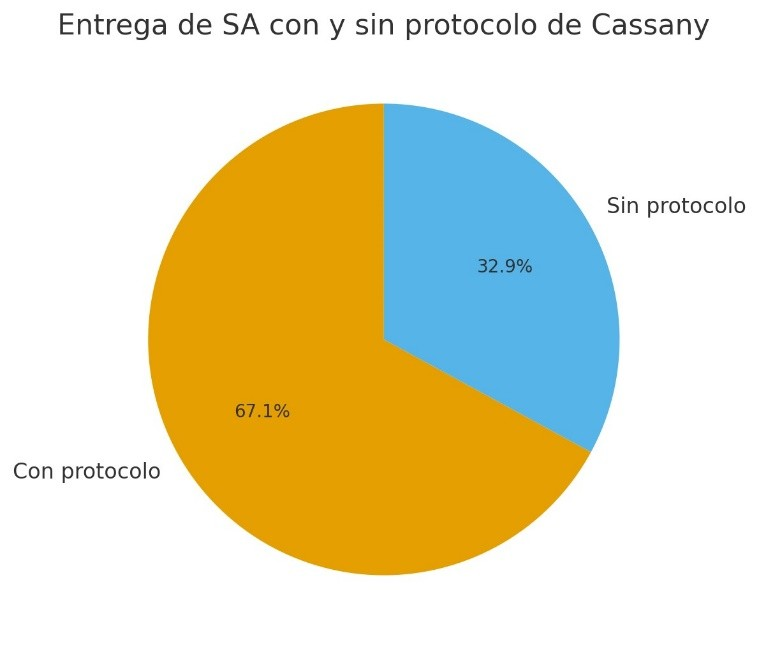
\includegraphics[width=\textwidth]{Figura 1.jpg}
% \caption{Resultados del alumnado al uso de la IA.}
% \label{fig1}
% \source{Elaboración propia.}
% \end{minipage}%
% \qquad
% \begin{minipage}{0.45\textwidth}
% 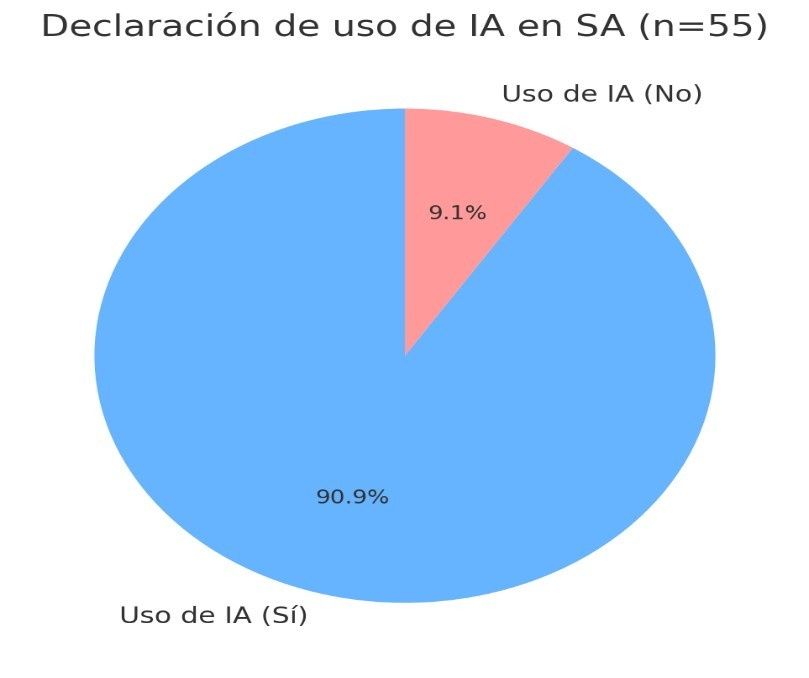
\includegraphics[width=\textwidth]{Figura 2.jpg}
% \caption{Resultados del alumnado al uso de la IA.}
% \label{fig2}
% \source{Elaboración propia.} 
% \end{minipage}%
%\end{figure}

\begin{figure}[h!]
\centering
\begin{minipage}{.6\textwidth}

\includegraphics[width=\textwidth]{Fig1.jpg}
\caption{Resultados del alumnado al uso de la IA.}
\label{fig1}
\source{Elaboración propia.}
\end{minipage}
\end{figure}

\begin{figure}[h!]
\centering
\begin{minipage}{.6\textwidth}

\includegraphics[width=\textwidth]{Fig2.jpg}
\caption{Resultados del alumnado al uso de la IA.}
\label{fig2}
\source{Elaboración propia.}
\end{minipage}
\end{figure}

Del total de 82 prácticas analizadas (correspondientes a 246 estudiantes), se observa en las respuestas una presencia significativa del uso de IAG en el diseño de las SA. La mayoría de estudiantes que responden emplea ChatGPT (84\%), seguida de Gemini (11\%); pero no se preguntó sobre este dato en particular. Debido a que ya existen trabajos respecto a qué IAG suele usar el alumnado \cite{MulaGrauSegarraSaavedraCambroneroSaiz2025} que coincidían en resultados con el estudio aquí presentado, se apostó por averiguar cómo usaban tales herramientas para la Didáctica. Aunque no todos los grupos la emplearon, buena parte de ellos reconoce haber recurrido a dicha tecnología en alguna fase del trabajo.

En cuanto a los usos más frecuentes, destacan tres ámbitos principales:

\begin{enumerate}
    \item Generación y adaptación de textos (cuentos, noticias, diálogos, descripciones de personajes, guiones para \textit{podcasts}, etc.).
    \item Apoyo a la evaluación (elaboración de rúbricas, listas de cotejo y criterios de valoración).
    \item Creación de recursos multimodales (imágenes, canciones, materiales visuales para alumnos con necesidades específicas).
\end{enumerate}

La bibliografía usada para verificar los resultados responde a referencias básicas para la Didáctica de la Lengua y la Literatura. No obstante, algunas referencias no existen. Resultan alucinaciones que no siempre son detectadas por el alumnado, por lo que verifican los resultados con referencias erróneas. Este es uno de los puntos que deben contrastar de cara a un uso ético de la IAG.

En cuanto a la personalización y el grado de aprendizaje, reconocen haber mejorado una serie de competencias para la didáctica mediante el uso de IAG. Especialmente, a partir del protocolo presentado.

Con base en las declaraciones del alumnado, se observa que el uso de la IAG no se limitó exclusivamente a la producción de textos escritos, sino que abarcó una diversidad de formatos y funciones. Los participantes emplearon estas herramientas para la creación, adaptación y revisión de textos narrativos, expositivos e instructivos, así como para el diseño de rúbricas de evaluación, guiones radiofónicos y \textit{podcasts}, la generación de imágenes educativas y, en algunos casos, la composición de recursos sonoros y canciones mediante plataformas específicas. En relación con las fuentes y referencias, los estudiantes manifiestan una actitud selectiva y prudente: reconocen explícitamente que no incorporaron la totalidad de los resultados generados por la IAG, especialmente cuando detectaron imprecisiones, falta de adecuación al nivel educativo o incoherencias con los objetivos didácticos, lo que evidencia procesos básicos de verificación y contraste. Asimismo, las reflexiones aportadas muestran indicios de personalización y aprendizaje, en la medida en que el alumnado describe la modificación sustancial de los textos generados, la adaptación al contexto del aula y al currículo oficial, y la toma de decisiones pedagógicas propias. En conjunto, estas prácticas apuntan a un uso predominantemente instrumental y complementario de la IAG, orientado a la generación de ideas, la optimización del tiempo y el apoyo al proceso creativo, sin que ello implique una delegación plena de la autoría ni del criterio docente en formación.

Los \textit{prompts} analizados reflejan que los estudiantes priorizaron funciones relacionadas con la redacción académica (“revisa este párrafo”, “mejora la coherencia del texto”), con la creatividad (“dame ideas originales para una actividad”) y con la inclusión educativa (“adapta este material para un niño con TDAH/TEA”). Asimismo, varios grupos solicitaron apoyo para adaptar contenidos complejos (como La Divina Comedia o temas de los ODS) al nivel de Primaria.

En el plano de la percepción estudiantil, emergen dos tendencias:

\begin{enumerate}
    \item Una visión instrumental y pragmática, que valora la IAG como recurso útil para agilizar tareas, encontrar ideas y mejorar la presentación de los trabajos.
    \item Una visión crítica y cautelosa, que subraya los límites de fiabilidad, la necesidad de contrastar con otras fuentes y el riesgo de dependencia excesiva.
\end{enumerate}

En general, los estudiantes reconocen que la IAG no sustituye la reflexión pedagógica ni la creatividad docente, más bien actúa como apoyo complementario. Muchos destacan la importancia de revisar y adaptar lo generado, y de mantener siempre el juicio profesional propio.

De tal modo se desglosan y categorizan los \textit{prompts}:

El análisis de los \textit{prompts} declarados por el alumnado permite identificar diferentes usos funcionales de la IAG, relacionados con las fases del proceso didáctico y de producción académica. En primer lugar, una parte significativa de los \textit{prompts} se orienta a la revisión y mejora de textos propios. En estos casos, el alumnado solicita a la IAG que revise, reformule o mejore la claridad, coherencia y adecuación formal de textos previamente elaborados. Este tipo de uso sitúa a la herramienta como apoyo al proceso de escritura y metacorrección, manteniendo el texto de partida y el control autoral en manos de cada estudiante.

Una segunda categoría agrupa los \textit{prompts} vinculados a la generación de ideas y a la planificación didáctica. Aquí se incluyen solicitudes destinadas a proponer temáticas, actividades, proyectos o enfoques creativos para SA en el área de Lengua. Estos \textit{prompts} aparecen especialmente en fases iniciales del trabajo y cumplen una función exploratoria, facilitando la lluvia de ideas y la organización preliminar de propuestas que posteriormente son seleccionadas, adaptadas o descartadas por el alumnado.

En tercer lugar, se identifican \textit{prompts} centrados en la producción de textos educativos base, como cuentos, noticias, guiones radiofónicos o textos expositivos dirigidos al alumnado de Educación Primaria. Aunque la IAG genera textos relativamente extensos, las reflexiones de los participantes indican que estos materiales suelen ser utilizados como borradores o modelos iniciales, que después son modificados sustancialmente para ajustarse al nivel educativo, a los objetivos didácticos y al enfoque pedagógico del proyecto.

Otra categoría relevante corresponde al diseño de instrumentos de evaluación. En este caso, los \textit{prompts} se orientan a la elaboración de rúbricas, criterios de evaluación o ítems para la coevaluación y la autoevaluación. El uso de la IAG se concibe como un apoyo técnico-pedagógico que ayuda a estructurar la evaluación, sin sustituir el criterio profesional del futuro docente, que selecciona y adapta los elementos propuestos.

Asimismo, se observa un conjunto de \textit{prompts} relacionados con la adaptación lingüística y la atención a la diversidad. Estos incluyen solicitudes para simplificar textos, ajustar el vocabulario, generar frases de apoyo para alumnado con desconocimiento de la lengua vehicular o proponer recursos accesibles para estudiantes con necesidades educativas específicas. Este uso revela una preocupación explícita por la inclusión y la adecuación contextual de los materiales.

Finalmente, se identifica una categoría vinculada a la generación de recursos multimodales, que abarca la creación de imágenes, ilustraciones, canciones o materiales sonoros mediante distintas herramientas de IAG. Estos \textit{prompts} se utilizan como complemento visual o auditivo de las situaciones de aprendizaje, con el objetivo de aumentar la motivación del alumnado y enriquecer las propuestas didácticas, y se describen mayoritariamente como un apoyo puntual y no central en el proceso de enseñanza-aprendizaje. La siguiente tabla (\Cref{tab2}) resume la categorización de \textit{prompts}.


\begin{table}[h!]
\centering
\begin{threeparttable}
\caption{Análisis de los protocolos de uso de IAG.}
\label{tab2}
\begin{tabular}{p{9cm}cc}
\toprule
\textbf{Eje de análisis} & \textbf{Casos} & \textbf{Porcentaje} \\
\midrule
Reconocimiento del uso de IAG & 50 & 61,0\% \\
Declaración de fines (respuestas rápidas) & 16 & 19,5\% \\
Declaración de fines (revisión/mejora) & 28 & 34,1\% \\
Declaración de fines (ideas originales) & 33 & 40,2\% \\
Declaración de fines (otros) & 14 & 17,1\% \\
Explicitación de prompts & 82 & 100\% \\
Verificación con fuentes externas & 5 & 6,1\% \\
Reflexión crítica & 82 & 100\% \\
\bottomrule
\end{tabular}
\source{Elaboración propia.}
\end{threeparttable}
\end{table}

Los resultados muestran un incipiente proceso de alfabetización crítica digital: si bien el alumnado en formación emplea la IAG de manera experimental, en la mayoría de los casos es consciente de sus sesgos y limitaciones, y demanda pautas claras para un uso ético y regulado en el ámbito educativo. Según los ejes planteados por Cassany, el análisis se sintetiza del siguiente modo:

\begin{enumerate}
    \item Transparencia en el uso de la IAG
    
    De las 82 Situaciones de Aprendizaje (SA) entregadas, recordemos, solo 55 (es decir, 165 personas; el 67\%) incluyeron el protocolo. En este caso, apenas 5 grupos (15 personas) declararon no haber utilizado la IAG, lo que significa que más del 90\% reconoció su uso en el diseño de la práctica. Este dato muestra una clara tendencia a normalizar la incorporación de la IAG en la formación docente, aunque persisten resistencias en la presentación explícita del protocolo.

    \item Declaración de los fines específicos perseguidos

    Los fines declarados fueron diversos, pero se pueden agrupar en tres grandes categorías:

    \begin{enumerate}
    \item Redacción y adaptación textual: creación de cuentos, guiones, noticias o descripciones; reescritura y mejora de la coherencia de los trabajos.
    \item Apoyo didáctico y evaluativo: generación de ideas para actividades, elaboración de rúbricas, propuestas de criterios de evaluación y adaptación de tareas a estudiantes con NEAE (TDAH, TEA, dislexia, alumnado extranjero).
    \item Producción multimodal: creación de imágenes, canciones y materiales visuales para enriquecer las SA.
    \end{enumerate}

    Esto refleja una visión de la IAG como herramienta flexible, tanto para resolver necesidades inmediatas como para expandir la creatividad docente, aunque en muchos casos queda la duda de cuál ha sido la contribución del alumnado en el ámbito creativo más allá de los resultados hallados por la IA.

    \item Explicitación de los \textit{prompts} empleados

    La mayoría de los grupos incluyó ejemplos de \textit{prompts}, lo que aporta transparencia sobre el tipo de interacción mantenida con la IAG. Estos \textit{prompts} oscilan entre peticiones simples (“Revisa este párrafo”) y solicitudes más complejas (“Diseña un cuento adaptado para un alumno con dislexia y otro extranjero”). En este sentido, los futuros docentes no solo usaron la IAG para microtareas, sino también para explorar escenarios de inclusión, creatividad y transversalidad en el diseño de actividades.

    \item Verificación de resultados mediante fuentes externas

    Aunque no todos los protocolos reportan un contraste explícito, sí se observa una tendencia a revisar y adaptar las respuestas generadas. Varios grupos subrayan la necesidad de comprobar la fiabilidad de la información en fuentes académicas o curriculares, y en algunos casos señalan directamente que no utilizaron todas las sugerencias de la IAG por considerarlas inadecuadas. Este hallazgo confirma lo advertido por Cassany (2024): la utilidad de la IAG depende de que el alumnado la complemente con un juicio crítico y pedagógico propio.

    \item Reflexión crítica sobre la influencia de la IAG en el trabajo académico

    En sus reflexiones, el alumnado muestra dos posturas principales:

    \begin{enumerate}
        \item Una visión instrumental y positiva, que valora la IAG como recurso de apoyo útil para agilizar procesos, ampliar ideas y facilitar la elaboración de materiales.
        \item Una visión crítica y precautoria, que reconoce los riesgos de error, incoherencia o dependencia excesiva, insistiendo en la necesidad de revisar, contrastar y mantener la autoría personal en el trabajo.
    \end{enumerate}
\end{enumerate}

En conjunto, estas reflexiones evidencian un incipiente proceso de alfabetización crítica digital, en línea con los planteamientos de \textcite{UbalCamachoTambascoMartinezGarciaCorrea2023,CervantesBarriosMonteceMoranteMeraMedina2024}, que destacan la importancia de enseñar no solo a usar tecnología, sino a cuestionarla y regularla; tal como se recoge en la \Cref{fig3}.

\begin{figure}[h!]
\centering
\begin{minipage}{.9\textwidth}
 
\includegraphics[width=\textwidth]{Fig3.jpg}
 \caption{Resultados por ejes de \textcite{Cassany2024}.}
 \label{fig3}
 \source{Elaboración propia.}
\end{minipage}
\end{figure}

La tabla y el gráfico de barras permiten observar con claridad la distribución de los resultados en torno a los cinco ejes planteados por \textcite{Cassany2024}. El primer dato destacable es que el 61\% de los protocolos reconocen explícitamente el uso de la IAG, lo que confirma su rápida incorporación en la formación docente. Este reconocimiento se acompaña de una diversidad de fines: el 40,2\% la emplea para generar ideas originales, el 34,1\% para revisar y mejorar los trabajos y un 19,5\% para obtener respuestas rápidas. Además, en un 17,1\% de los casos aparecen usos clasificados como “otros”, entre los que figuran la creación de imágenes, canciones y materiales de apoyo para alumnado con necesidades específicas.

En relación con los ejes de transparencia y autorregulación, destaca que en varios protocolos se consignan ejemplos de \textit{prompts}, lo que muestra un ejercicio de explicitación que va en línea con la propuesta de \textcite{Cassany2024}. Sin embargo, la verificación con fuentes externas aparece de manera más limitada, lo que evidencia que todavía no se ha consolidado una práctica sistemática de contraste de la información.

El gráfico de barras sintetiza estas tendencias al situar en primer plano la función creativa y de apoyo a la redacción de la IAG, mientras que deja en segundo plano el eje de la verificación. Este desequilibrio refuerza la necesidad de insistir en la alfabetización crítica digital, ya que el alumnado reconoce la utilidad de la IAG pero no siempre la acompaña de procedimientos sólidos de control y validación de la información.

En conjunto, los datos muestran un alumnado en proceso de apropiación crítica de la IAG: consciente de su potencial para enriquecer la práctica docente, pero aún en construcción respecto de los hábitos de evaluación y transparencia necesarios para garantizar un uso ético y responsable.

El análisis de los protocolos a partir de los cinco ejes de \textcite{Cassany2024} permite comprobar que, si bien cada dimensión ofrece una mirada clara sobre el uso de la IAG en la formación docente, la categoría relativa a la declaración de fines específicos se ramifica en varias subdimensiones que enriquecen y complejizan el marco inicial. En efecto, los resultados muestran que el alumnado no declara un único fin; ya que diferencia entre la búsqueda de respuestas rápidas a dudas concretas (19,5\%), la revisión y mejora de la redacción y coherencia de los trabajos (34,1\%), la obtención de ideas originales y creativas (40,2\%) y, en menor medida, otros usos diversos (17,1\%), como la creación de imágenes, canciones o materiales inclusivos. Esta diversificación de propósitos evidencia que el eje propuesto por Cassany no se agota en la mera identificación de una finalidad genérica; es decir, requiere una lectura ampliada que dé cuenta de la pluralidad de funciones que las y los futuros docentes atribuyen a la IAG. Dicho de otro modo, la ramificación de este eje permite observar cómo la herramienta no solo actúa como apoyo mecánico —al agilizar tareas rutinarias o de redacción—, sino que también se convierte en catalizador de procesos creativos, inclusivos y multimodales, vinculados directamente con la innovación didáctica. Al ampliar este eje, se hace visible que la IAG desempeña simultáneamente un papel instrumental y uno estratégico en la práctica académica: facilita la resolución de problemas inmediatos, pero también abre posibilidades pedagógicas que dialogan con las competencias clave y con la necesidad de una educación lingüística crítica y contextualizada. Ahora bien, existe un riesgo de que el alumnado confíe la innovación y los procesos creativos a la IAG, puesto que eso significaría el estancamiento de dichos procesos.


\section{Discusión}\label{sec-organizacao-latex}
Los resultados obtenidos muestran una aceptación mayoritaria del uso de la IAG en la formación inicial del profesorado de Primaria. De los 55 protocolos analizados, únicamente 5 afirman no haber recurrido a estas herramientas, lo que confirma la rápida incorporación de la IAG a las prácticas académicas. Sin embargo, el hecho de que 27 grupos no incluyeran el protocolo de Cassany en sus entregas revela resistencias a explicitar y transparentar dicho uso, lo que coincide con lo planteado por Cassany (2024), quien subraya la necesidad de generar espacios de confianza y de asumir la IAG desde una perspectiva formativa más que punitiva.

Estos hallazgos se alinean con investigaciones previas que destacan tanto el potencial como las tensiones que genera la IAG en contextos educativos. \textcite{SanchezVera2024} ya señalaba que el profesorado en formación reconoce en la IA un recurso de apoyo para la creación textual, la revisión y la adaptación de materiales, mientras que \textcite{RoviraColladoMartinezCarratalaMiras2024} enfatizan el desafío de situar estas herramientas dentro de la Didáctica de la Lengua y la Literatura, sin reducirlas a un mero soporte técnico. En este estudio, los futuros docentes declaran haber utilizado la IAG especialmente para redactar cuentos, adaptar textos, elaborar rúbricas y diseñar recursos multimodales, lo que evidencia un uso diverso, pero todavía incipiente en términos de integración pedagógica.

Al mismo tiempo, el alumnado manifiesta una actitud crítica y vigilante: aunque reconoce la utilidad instrumental de la IAG (optimización de tiempo, generación de ideas, apoyo a la evaluación), también advierte sus limitaciones (errores, falta de adecuación, riesgo de dependencia). Esta ambivalencia coincide con lo reportado por \textcite{MartinMarchante2022,Gragera2024}, quienes observaron una relación de utilidad-desconfianza en estudiantes universitarios, y con \textcite{Lindin2024}, que documenta la necesidad de acompañamiento docente para desarrollar un uso consciente y autorregulado.

La discusión también debe situarse en el marco de la alfabetización crítica digital \cite{UbalCamachoTambascoMartinezGarciaCorrea2023,CervantesBarriosMonteceMoranteMeraMedina2024}, que demanda enseñar a manejar herramientas tecnológicas al tiempo que se cuestiona su fiabilidad, sesgos y efectos sociales. El hecho de que la mayoría del alumnado reflexione sobre la influencia de la IAG en sus prácticas indica un avance en este sentido, aunque la ausencia de protocolos en un tercio de los casos muestra que todavía falta consolidar una cultura de transparencia en el uso académico de estas tecnologías.

En conjunto, tales resultados aportan evidencia a la discusión internacional sobre la incorporación ética de la IAG en la enseñanza de lenguas. Confirman la pertinencia de protocolos estandarizados como los ya citados, al tiempo que sugieren la necesidad de diseñar estrategias de acompañamiento docente que permitan a los futuros maestros usar la IAG.

\section{Conclusión}

El estudio confirma que la Inteligencia Artificial Generativa (IAG) se ha incorporado de forma acelerada en la formación inicial del profesorado de Primaria. La mayoría del alumnado reconoce haber recurrido a estas herramientas para el diseño de Situaciones de Aprendizaje, especialmente en tareas de redacción, adaptación de materiales, elaboración de rúbricas y creación de recursos multimodales. Sin embargo, la ausencia del protocolo en un tercio de las entregas revela que todavía persiste cierta resistencia a transparentar este uso, lo que subraya la importancia de seguir trabajando en la construcción de una cultura académica de honestidad y ética digital.

La investigación evidencia también que el alumnado mantiene una postura ambivalente ante la IAG: la percibe como un apoyo eficaz para ahorrar tiempo y generar ideas, pero al mismo tiempo advierte de sus limitaciones y la necesidad de verificación constante. Este doble enfoque muestra un incipiente proceso de alfabetización crítica digital, en el que la reflexión sobre el uso de la IAG se convierte en una competencia clave para la docencia del siglo XXI.

De cara al futuro, resulta imprescindible avanzar en la implementación de protocolos estandarizados, como el que hemos adaptado a partir de \textcite{CassanyCasarin2025}, que permitan regular el uso de estas herramientas en contextos universitarios y formar al profesorado en prácticas críticas, responsables y éticas. Asimismo, se recomienda ampliar la investigación a otros niveles educativos y disciplinas, con el fin de consolidar una visión más amplia sobre las posibilidades y los límites de la IAG en la educación lingüística. En dicha línea se planea de cara a futuras investigaciones un estudio comparativo entre tercer y primer curso.

Los resultados de esta investigación evidencian que la IAG no es ya un fenómeno externo a la educación. Se trata de una herramienta que atraviesa las prácticas de formación docente y redefine la manera en que se conciben la SA. El alumnado universitario no solo la emplea para redactar o corregir textos, sino que también la integra en procesos de evaluación, inclusión y producción multimodal, lo que confirma que la IAG se encuentra en la intersección entre la educación lingüística, la multimodalidad y el discurso. Sin embargo, consideramos que el verdadero reto es que el propio alumnado realice contribuciones que vayan más allá del alcance de los resultados obtenidos por la propia IAG y no se limite a aceptarlos en el terreno de la creatividad y la innovación, puesto que esto reduciría su propia voz y condicionaría, como afirman \textcite{MagroLara2025}, su capacidad de crear respuestas más libres o disruptivas, estancando así el propio proceso.

En relación con el análisis cualitativo, conviene explicitar que las reflexiones del alumnado fueron categorizadas a partir de un proceso de análisis inductivo, centrado en la finalidad atribuida a la IAG y en el grado de intervención personal declarado. Las categorías emergieron del examen reiterado de las respuestas, atendiendo a aspectos como el tipo de tarea en la que se empleó la herramienta, el nivel de modificación de los resultados generados, la presencia de procesos de verificación y contraste, y las referencias explícitas al aprendizaje o a la toma de decisiones pedagógicas. Esta estrategia permitió identificar patrones recurrentes en los discursos estudiantiles y agrupar las reflexiones según funciones dominantes de apoyo a la escritura, generación de ideas, creación de recursos, evaluación, adaptación lingüística o producción multimodal, sin perder de vista la diversidad de prácticas individuales.

Desde una perspectiva formativa, la explicitación de dichas categorías contribuye a una mejor comprensión del modo en que el alumnado en formación inicial del profesorado se apropia de la IAG de manera mayoritariamente instrumental, reflexiva y contextualizada. Las conclusiones del estudio muestran que el protocolo de uso ético y transparente favorece la autorregulación y la conciencia crítica, al tiempo que también proporciona un marco analítico para interpretar las reflexiones estudiantiles con mayor claridad y rigor. En dicha línea, el trabajo refuerza la necesidad de integrar la reflexión guiada sobre el uso de la IAG en la enseñanza universitaria: más que como un mero requisito declarativo, se trata de aprovechar una oportunidad para el desarrollo de competencias profesionales vinculadas a la toma de decisiones pedagógicas responsables y a una educación lingüística crítica. De ese modo, el alumnado que pronto será docente, de Primaria, dominará una serie de herramientas que le permitirán llevar a cabo el proceso de enseñanza-aprendizaje de acuerdo al contexto en el que encontrará de igual modo su alumnado. El diseño de la SA le permitirá evaluar las competencias sin depender de un uso fraudulento de la IAG. Se conocerá, pues, cuáles son las posibilidades éticas que esta plantea, tal como se ha evidenciado en la reflexión tras el protocolo utilizado.

Al mismo tiempo, las resistencias a declarar su uso y la limitada verificación de resultados revelan que aún queda camino por recorrer en la construcción de una cultura crítica y ética. La IAG se presenta así como un espejo de las tensiones contemporáneas entre innovación tecnológica y responsabilidad social: su potencial es innegable, pero su apropiación plena depende de la capacidad de formar docentes capaces de interrogar, contextualizar y reconfigurar sus usos en diálogo con los marcos legales, éticos y pedagógicos.

En este sentido, el estudio contribuye a las líneas del dosier al mostrar que la IAG no solo impacta la vida social mediante nuevas formas de interacción; también transforma la educación lingüística al ampliar las posibilidades expresivas, creativas e inclusivas. Asimismo, su carácter multimodal y su poder para generar discurso sitúan a la IAG en el centro de un debate ineludible: cómo convertirla en un recurso de emancipación crítica y no en un dispositivo de dependencia acrítica. La conclusión es clara: la formación docente es el espacio privilegiado para ensayar este tránsito.

\printbibliography\label{sec-bib}
% if the text is not in Portuguese, it might be necessary to use the code below instead to print the correct ABNT abbreviations [s.n.], [s.l.]
%\begin{portuguese}
%\printbibliography[title={Bibliography}]
%\end{portuguese}


%full list: conceptualization,datacuration,formalanalysis,funding,investigation,methodology,projadm,resources,software,supervision,validation,visualization,writing,review
\begin{contributors}[sec-contributors]
\authorcontribution{Natalia Contreras-de la Llave}[conceptualization,formalanalysis,investigation,methodology,projadm,writing]
\authorcontribution{Ignacio Ballester-Pardo}[conceptualization,resources,validation,supervision,visualization,review]
\end{contributors}

\begin{dataavailability}
\txtdataavailability{dataavailable} % options: dataavailable, dataonly, databody, datanotav, nodata
\end{dataavailability}

\appendix 
\section{Anexo 1}\label{apx-longtable}
En los siguientes enlaces pueden encontrar los datos de la investigación. En primer lugar, los \textit{prompts} del alumnado:

\url{https://docs.google.com/document/d/1w8ENNpejwfBetqbYdFBfZRXiutkNf5G7/edit?usp=sharing&ouid=113597142270018182869&rtpof=true&sd=true}

Y, en segundo lugar, los resultados de los 82 grupos analizados:

\url{https://docs.google.com/spreadsheets/d/1PFhCcR9vvkq2jdafTwM06CoY9BHnsOuFQB0MZUVknWk/edit?usp=sharing}


\end{document}

